\documentclass[a4paper]{article}

\usepackage{url}
\usepackage{listings}
\usepackage{graphicx}
\graphicspath{ {images/} }

\newcommand{\subsubsubsection}[1] 
{
	\paragraph{#1}
	\mbox{}\\
	
	\noindent
}

\setcounter{secnumdepth}{5}	
\setcounter{tocdepth}{5}

\lstloadlanguages{C++}
\lstset{language=C++, breaklines=true}


\title{Isometric Hack and Slash Game Engine}
\author{Tom Mason - 10329877\\Supervisor: Mads Haahr}

\begin{document}
\maketitle

\begin{abstract}
The purpose of the project is to create a modern open source reimplementation of the engine used in the 1996 video game Diablo.\\
It will use the original data files, so as to avoid issues with copyright, but will also
support modern file formats, and be a generic engine for games of that style.\\
The original game is an isometric top down hack and slash game, which features some roguelike elements, such as
random items and dungeons. These will be a focus of the project.
\end{abstract}

\newpage

\tableofcontents

\newpage

\chapter{Related work}
In this chapter I will attempt to review a number of projects similar to this one. They will be evaluated based on their perceived usefulness to this project, which is comprised of: licensing, embedded scripting language, networking support and code quality.

    	\section{Flare Isometric Engine}
    	Flare\cite{flare} is an open source isometric hack and slash game engine. It uses the SDL library for displaying graphics, and simple text based file formats. It is in active development at time of writing, and is available under the GPLV3.
    	It does not appear to have any embedded scripting language.
    	
    	\section{Holyspirit}
    	Holyspirit\cite{holyspirit} claims to be in alpha. It uses the SFML library. Does not appear to support networking.
    	Developed in French. Unlike the above, it is an actual game in the hack and slash genre, as opposed to a game engine (although an engine is, of course a part of it). It is also available under a permissive license.
    	
    	\section{Fifengine}
    	Fifengine\cite{fife} (Flexible Isometric Free Engine) is a FOSS generic isometric game engine.
    	It supports python scripting, and the UI is skinnable with xml.
    	It uses SDL and opengl. It does not support networking.
    	Like Flare, it is a game engine, not a game, but it is more generic, in that is is intended for all kinds of isometric games.
    	
    	\section{ProjectDDT}
    	ProjectDDT\cite{ddt} is an existing attempt to create a modern FOSS engine for Diablo.
    	It has been abandoned now since 2011.
    	Extending this project was considered over creating a new one, but this was decided against as the existing code appears unmaintainable and quite hard to follow.
    	It is however, very useful as a reference, as it is under the GPL.
    	It contains code for loading and interpreting several diablo file formats which proved useful.
    	
    	\section{Diablo 1 HD Mod}
    	This\cite{d1hd} is another recreation of the diablo engine that is far more advanced than ProjectDDT. The game appears to be fully playable. However, the source code is not available, and there does not appear to be any plans for it to be made available at any point.
	
\newpage
        
  \section{Design Choices}
    The engine should support python scripting, to allow entension of the engine, and of games created forthe engine.
    File formats used by the game should be simple text formats, like the formats used in Fifengine.
    The engine should be divided into a number of module.
    
    \subsection{Architecture}
    Then architecture of the engine has been based on the OpenMW\cite{openmw} engine, with which I have some experience.
    The project produces a number of executables (currently the main engine executable, an image viewer, and a test program for the IO library), each having it's own subdirectory in the apps/ folder in the root of the project.
    
    Code common to multiple "apps" is placed in the components/ sudirectory in the root of the project, and external libraries that have to be shipped as source along with the engine source are placed in the extern/ folder.
    
    \subsection{Engine Architecture}
    Code withing the main engine folder is split into components prefixed with FA for freeablo. Again, this convention is borrowed from OpenMW\cite{openmw}.
    The main important components so far are:
    \begin{itemize}
        \item{FAWorld - a container object for the state of the current level. Holds all the objects on the level, and is responsible for updating them (i.e moving them around in response to input etc.)}
        \item{FALevelGen - responsible for generating random dungeons}
        \item{FARender - controls rendering to screen}
    \end{itemize}

    \subsection{Renderer}
    The current rendering library being used is SDL 1.2. However, all SDL specific code has been confined to two files, with all other parts of the code using functions exported by those two files. This is done with the intention of easing the transition of switching to SDL 2 in the future.
    
    Rendering code is split into two parts, in different places. There is a rendering "component" in the components/render folder.
    This component exports basic rendering functions for loading and drawing sprites etc, but does not deal with the rendering loop, it has a draw() function which will swap the buffers, and must be called manually.   
    It is essentially a wrapper for a low level rendering library, with some application specific logic (it has the ability to draw "levels", ie Level::Level objects representing an isometric level of the game, and also load the proprietary CEL and CL2 formats).
    This code is placed in a component because it is common to both the freeablo game engine and the image viewer.
    
    \mbox{}
    
    The second part is the code that controls the actual rendering for the game. This is located in apps/freeablo/farender. Essentially, this contains a class FARender::Renderer, that manages sprite loading and render looping for the game engine.  
    When created, the Renderer class starts up a seperate thread, which then loops until the object is destroyed. Each iteration, the renderer will draw the level, and a list of objects, which are essentially just sprites and locations.
    The game engine communicates with the renderer through a triple buffered system.
    
    The Renderer creates three RenderState objects, each of which is just a container for a number of sprites and their corresponding locations, and a location on which to centre the camera.
    Each iteration of the game loop, after processing the game logic for the current tick, the engine will "fill" a render state, and pass it off to the renderer. This filling is basically just a flattening of game state, removing all information about objects other than sprite and location, and dumping it into the state.
    Three states are used, as at any given point the renderer can be drawing a state, and the game loop can be filling one, so with three we are always guaranteed to have one free.
    Locks are used when rendering and filling a state to ensure that we are never reading and writing the same state at the same time.
    As the game and render loops can (and probably are) iterating at different rates, when the render loop is going faster, some render states will never be drawn to screen, but this is ok as whatever is on screen at any given moment is an accurate portrayal of game state to the granularity allowed by the iteration speed of the renderer, which is determined by the speed of your processor and GPU (no framelimit is set on the renderer).
        
    \subsection{Input}
    Input is handled in the main thread. Like rendering, it is done using SDL, so it is also abstarcted away in the Input compnent.
    The input component consists of an object to which one binds callbacks. These callbacks are then executed when the poll() method is called, if the corresponding input actions have occurred.

    
    \subsection{Libraries}
        \subsubsection{2d graphics libraries}
    	There seems to be 3 different options for 2d graphics in C++:
    	\begin{itemize}
    	    \item{SDL}
    	    \item{Allegro}
    	    \item{SFML}
    	\end{itemize}
    	
    	Of the above, all are written in plain C, except Allegro, which is C++.
    	I have decided to use SDL for this project, as I am already familiar with it.
    	More specifically, I have decided to use SDL 1.
    	SDL 2 has been released, but is not yet packaged in most distros. 
    	The intent is to write an SDL backend, which will eventually support either SDL1 or 2.
    	
    	\subsubsection{Cross Platform}
        The Boost C++ library addressess many of the problems with writing portable C++ code today.
        Specifically, I intend to make use of the boost::filesystem and boost::threads modules to provide platform-agnostic access to threads and files.
        Even with bo	ost::filesystem, I shall have to take care to use case insensitive file loading, as the original game was written for windows, so filename cases may not be consistent.
        
        \subsubsection{Audio}
        SDL has a module for audio, SDL\_sound\cite{sdls}, but it has not been updated since 2008.
        FFMPEG's library, libavcodec\cite{libavcodec} supports a lrge number of formats.
        OpenAL seems to be popular also, but is no longer FOSS.
\newpage
	
\section{Level Generation}
    Level generation in freeablo is performed in a number of stages. The first stage is the creation of a flat map. This is the part with interesting alorithms.
    After that, the map is turned isometric, and then has monsters place + random variance introduced into the tileset, but neither of these are worth discussing.

    \mbox{}

    The level generation algorithm used in freeablo is borrowed from a game called TinyKeep\cite{tinykeep}, the author of which has published the algorithm he developed\cite{tinygen}.
    The algorithm is designed to create rooms connected by corridoors on a grid.
    There are a number of steps which are executed in sequence to produce this map.
    \begin{itemize}
        \item
        {
            The first step is to place a number of rooms in the centre of the grid, keeping them within a small circle placed there.
            The rooms can overlap within this circle, and indeed are expected to. The number of rooms, and the radius of the circle in which they are placed
            should be related in some way to the size of the map being generated. The width, height, and position within the circle of the rooms is randomly generated, with the randomness for width and height biased so we receive more small rooms than large ones.    
        }
        \item
        {
            After this, we use seperation steering to move the rooms away from eachother until none of them overlap.
        }
        \item
        {
            At this point, we split the rooms into two groups, by thresholding on size. Those over the threshold value (area of 30 was usind in the freeablo engine) are said to be real rooms, and the rest are said to be corridoor rooms. The bias when generating levels mentioned above ensures that most rooms are chosen to be corridoor rooms.
        }
        \item
        {
            We construct a graph of real rooms, where each rooms is connected to each other room. We then calculate the miniumum spanning tree of this graph. Now we know that if we apply corridoors corresponding to the edges on this graph, each room will be accessible from each other one.
        }
        \item
        {
            Becuase the graph we constructed above is a tree, there will be no cycles, however a small number of cycles is desirable in a dungeon crawler, so we add in a number of random edges to create some.
        }
        \item
        {
            For every edge on the graph, we create an l-shaped corridoor on the map, joining the two rooms that correspond to that edges vertices.
            This is where the corridoor rooms come into effect. For each corridoor room that the corridoors intersect, we add the shape of that room onto the corridoor. In this way, we end up with lumpy corridoors that can resemble large rooms themselves, and do not just look like simple l shapes.
        }
    \end{itemize}
\newpage

\section{File Formats}
In the following section, I will use stdint.h style names for naming datatypes with exact bit width.

\subsection{PAL files}
    PAL files are colour pallettes used by the image formats in diablo. They always contain 256 colours, and each colour is 3 bytes long (r, g, and b bytes), so they are always 768 bytes long. Image files refer to them by index into the file (so, a two would represent the 3rd colour, or the third group of three bytes).

\subsection{CEL image files}
	CEL image files use the CEL and CL2 file extensions. There are some minor differences between the two, but they are fundamentally the same. The basic capabilities of the format are run length encoding, and transparency (but only total transparency, not partial). Each file can contain multiple frames that can represent parts of an object, frames in an animation, or even tilesets for levels.

	\subsubsection{File Header}
	\label{sec:fileheaders}
	The file header is composed of a series of uint32\_t. The first is the number of frames. This is followed by an offset from the start of the file for each frame, and finally, an offset to the end of the file. Illustrated below is a pseudo-C struct representing it's structure.
	\begin{lstlisting}
struct fileHeader
{
	uint32_t numFrames;
	uint32_t frameOffsets[numFrames];
	uint32_t endOffset;
};
	\end{lstlisting}
	 This header is common to both CEL and CL2 files.
	 
	\subsubsection{Frame Headers}
	\label{sec:frameheaders}
	Some CEL frames contain headers at the start of the frame. It is 5 uint16\_t (10 bytes) long. Entries appear to be pointers to positions in the file, which when reached during decoding will leave us with a specific number of lines created, but I only understand the second entry (and it is the only one of use to us). This entry gives us a position in the file, that when we reach it, we will have processed 32 lines of pixels in the image. By checking how many pixels have been genrated by the time we get to that point, we can divide this number by 32 to get the image width.
	The first entry is always 10, as it points to the start of the image data.
	The third entry may point to the end of the 64th line (if it exists) and so on, but I have not investigated this as it is of no use to me.
	
	\subsubsection{CEL Frames}
	There are two kinds of plain CEL frame. One is the "normal" kind, which contains animations of objects. Examples of these can be found in the items directory in DIABDAT.MPQ. The other is tileset cel frames. As the name implies, these contain the tilesets for levels. These are found only in levels/*/*.cel.
	A given CEL file will only conatin one of these types, not both.
A colour in a CEL frame will always be a single byte index into a palette.

	\subsubsubsection{Normal CEL Frames}
	Normal Frames are composed of a series of command and data blocks.
	Each block is a uint8\_t.
	The command blocks contain instructions about what to do next during decoding. The data blocks contain indices into a palette to obtain a colour value.
	
	Decoding is performed by starting at the start of the file (the first block will always be a control block), and executing the command there. 
	\\Then you advance by the number of blocks specified by the current block, which brings you to the next control block, and so on until you have decoded the entire frame. There are two kinds of control block: Regular and Transparency.
	
	\emph{Regular blocks} are denoted by values $\leq 127$. When you encounter a regular block, it's value indicates how many pixels it contains. For example, if you encounter a Regular block with value 10, the next 10 blocks are data blocks, one pixel each, and the 11th block after is the next control block.
	
	\emph{Transparency blocks} are denoted by values $> 127$. When a transparency block is encountered, it indicates $256-$block value transparent pixels. Transparency blocks do no use any data blocks, and so the immediate next block is the next control block.
	
	Below is a sample implementation of decoding a frame.
	
	\begin{lstlisting}
// Frame is the raw frame from the file, pal is a palette
// raw_image is the destination for decoded pixels
void CelFile::normal_decode(vector<uint8_t>& frame, Pal pal, vector<colour>& raw_image)
{
    size_t i = 0;
    
    for(; i < frame.size(); i++)
    {   
        // Regular command
        if(frame[i] <= 127)
        {    
            size_t j;
            // Just push the number of pixels specified by the command
            for(j = 1; j < frame[i]+1 && i+j < frame.size(); j++)
            {
                int index = i+j;
                uint8_t f = frame[index];
                colour col = pal[f];
                raw_image.push_back(col);
            }
    
            i+= frame[i];
        }

        // Transparency command
        else // >= 128
        {
            // Push (256 - command value) transparent pixels
            for(size_t j = 0; j < 256-frame[i]; j++)
                raw_image.push_back(transparentColour()));
        }
    }
}
	\end{lstlisting}

\subsubsubsection{Tileset CEL frames}
	These CEL files have the same format as normal CEL files, but the data in the franes is different. There are a number of possible "types" of frame within tileset CEL files. All of them are always of width and height 32.
\begin{itemize}

	\item{Raw:} Raw frames are just that, 32*32=1024 bytes of raw colours, with no transparency. 
	
	\item{Normal:} Some frames are normal frames as described in the previous section. These never have headers when contained in tilese CEL files.
	
	\item{Greater/Less than frames:} These are the most interesting frame type in cel files. They are the tiny triangles which make up half of an isometric block on the map. The name greater/less than is borrowed from ProjectDDT\cite{ddt}. \\

\includegraphics{ltgt}\\ Above is an example of a less than and greater than frame respectively. As you can see, when placed together, they make up a 64*32 pixel isometric block.\\
You can tell if a frame is a less than or greater than frame by looking at the contents. A certain set of bytes will be zeroed in both cases.\\
Less Than: bytes 0,1,8,9,24,25,48,49,80,81,120,121,168,169,224,225\\
Greater Than: bytes 2,3,14,15,34,35,62,63,98,99,142,143,194,195\\

	These bytes are clearly in pairs. Each pair marks the end of two rows of colour, as shown in the image below:\\
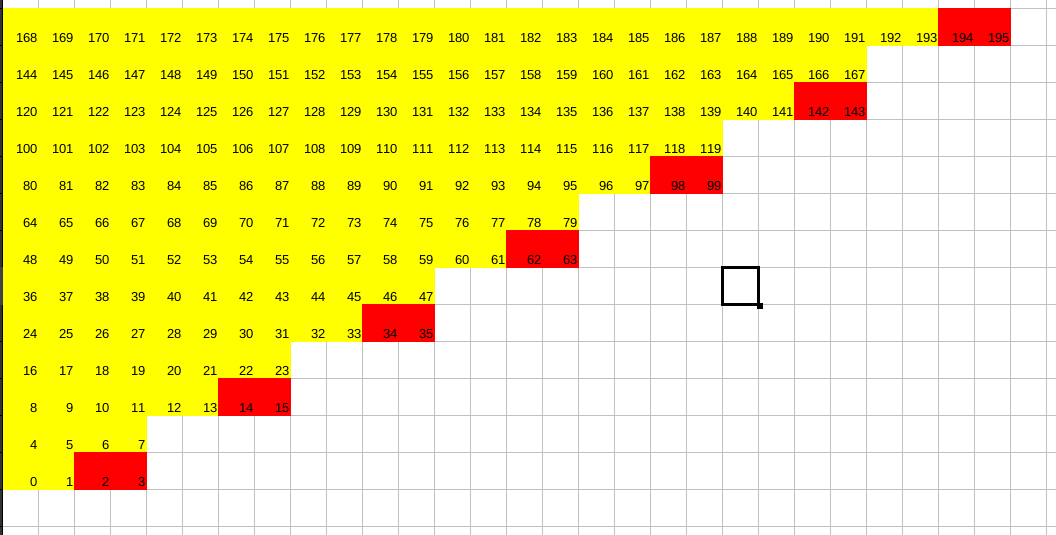
\includegraphics[scale=0.3]{ltgt-markers}\\
The yellow blocks are the bytes in between the markers, which contain colour indices, the red are the markers themselves. When rendereing, these are ignored, so all non-yellow blocks are transparent.

	For a given less/greater than frame, the first half will always conform to the scheme described above, but this only shows half the image.
	From there, there is variation. Some frames will have another half encoded the same way, with the following markers:\\
	Less Than Second Half: bytes 288,289,348,349,400,401,444,445,480,481,508,509,528,529\\
	Greater Than Second Half: bytes 245,255,318,319,374,375,422,423,462,463,494,495,518,519,534,535\\
	
	If these markers are not present, however, the second half is raw with no transparency, so we can just pull it out directly, eg:\\
	
\includegraphics[scale=0.5]{rawtop}
\end{itemize}

\newpage

\subsubsection{CL2 Frames}
	CL2 Frames are very similar to CEL frames, with the main difference that the use run-length encoding for colours as well as tranparency. They also always have frame headers.
   In addition to the regular and transparency blocks used in normal CEL frames, they also have RLE blocks, which indicate the number of times to repeat the colour indicated by the next block.
   Below is some C++ code that illustrates this:
   
   \begin{lstlisting}
void cl2Decode(const std::vector<uint8_t>& frame, 
   const Pal& pal, std::vector<Colour>& rawImage)
{
    size_t i = 10; // CL2 frames always have headers

    for(; i < frame.size(); i++)
    {
        // Color command
        if(frame[i] > 127)
        {
            uint8_t val = 256 - frame[i];
           
            // Regular command
            if(val <= 65)
            {
                size_t j;
                // Just push the number of pixels specified by the command
                for(j = 1; j < val+1 && i+j < frame.size(); j++)
                {
                    int index = i+j;
                    uint8_t f = frame[index];

                    Colour col = pal[f];

                    rawImage.push_back(col);
                }
              
                i+= val;
            }

            // RLE (run length encoded) Colour command
            else
            {
                for(int j = 0; j < val-65; j++)
                    rawImage.push_back(pal[frame[i+1]]);
          
                i += 1;
            }
        }
        
        // Transparency command
        else
        {
            // Push transparent pixels
            for(size_t j = 0; j < frame[i]; j++)
                rawImage.push_back(Colour(255, 0, 255, false));
        }
    }
}
   \end{lstlisting}
   
   As can be seen above, the blocks use different values, but the basic structure is the same as CEL frames.
   
 	\subsubsection{Frame Width}
 	Frame width determination is not as simple as it might sound. None of the frame formats have image dimensions built in, but there are a number of heuristics to find them.
 	For images with a frame header, the technique described in section \ref{sec:frameheaders} can be used. 
 	For tileset frames, the width is always 32.
 	For all others, there is another technique, which will work so long as the image width is not a multiple of 127, on images with no transparency (which headerless images seem to be).
 	
 	The maximum stretch of a Regular block is 127. A block will never straddle two lines, so if for example a frame were of width 130, there would be a series of 127 blocks followed by 3 blocks, one pair for each line.
 	
 	We can abuse this fact, by starting at the start of the frame, and adding together each command block until we find one that is not 127. At that point the sum of the previous 127s + the current block is the width of the image, as the current block has to exist to split on a line.
 	
 	\subsubsection{CEL Archives}
 	Some CEL and CL2 files are in fact archives of multiple CEL/CL2 files, respectively. These are used to store multiple rotations of an animation (eg walk animation in all 8 possible directions). These files have headers at the start, which consist of a number of uint32\_t s, each one pointing to a file contained in the archive.
 	
 	As there is always 8 images in such files, the first pointer will always be 32, as it will always point to the first byte after the headers, which are 8*4=32 bytes long, so it is possible to tell which files are archives by checking the first uint32\_t against 32.
 	
 	For CEL files, that's all there is to it, but for CL2, it's a little more complicated. The archive header on CL2 archives points not to the data, but to the individual file headers (described in section \ref{sec:fileheaders}), which then point to the frames, relative to their own position.

\newpage

\subsection{Level Files}
    Levels in diablo are stored in a number of files. To begin with, there is the heirarchy of DUN, TIL and MIN files.
    DUN files are the top level map file, which contain blocks that refer to the corresponding TIL file. Each entry in the TIL file is for tiles on the map, and each of those tiles is defined in the MIN file. The MIN file defines the sprites that make up the tile (total of 16). This is illustrated in the image below:\\
    
    \begin{center}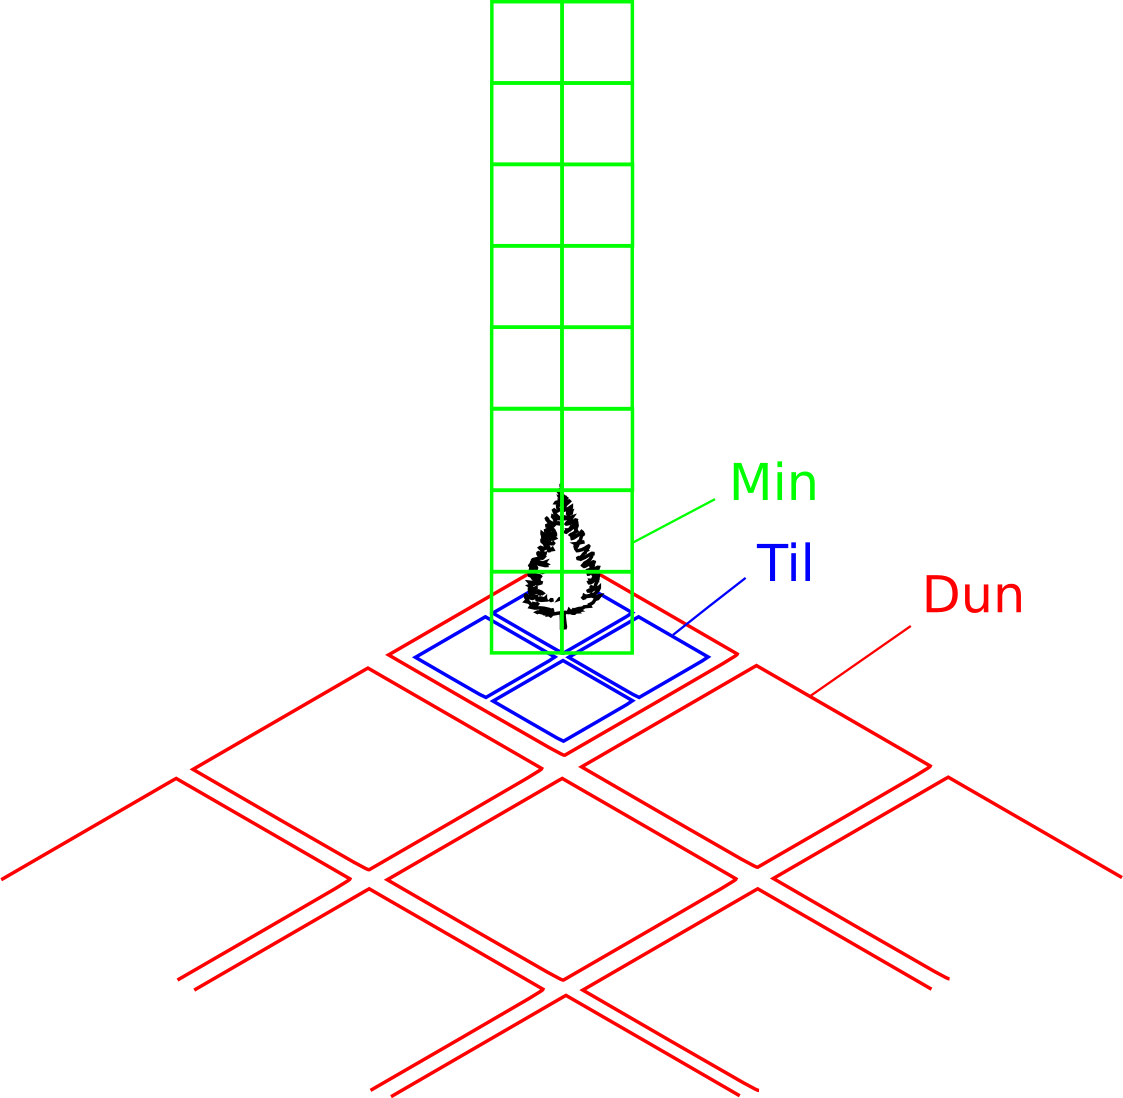
\includegraphics[scale=0.6]{level}\end{center}
    
    The properties of each tile is defined in the SOL file.

    \subsubsection{DUN files}
    DUN files are quite simple. They are essentyially a giant array of int16\_t s. The first two numbers are the width and height of the level (divided by four, as each block in the dun represents four actual level tiles). The remaining numbers are indices into the TIL file for each group of four tiles. Below is a c-style struct representing the structure of a dun file.
    \begin{lstlisting}
struct Dun
{
    int16_t width;
    int16_t height;
    int16_t blocks[width][height];
};
    \end{lstlisting}

    \subsubsection{TIL files}
    TIL files are also quite simple. they are just a massive array of int16\_t s, where each group of four is a block that can be referred to by the DUN file.

    \begin{lstlisting}
struct TilBlock
{
    int16_t top;
    int16_t left;
    int16_t right;
    int16_t bottom;
};

struct Til
{
    TilBlock blocks[FILESIZE/4];
};
    \end{lstlisting}

    \subsubsection{MIN files}
    MIN files are slightly awkward in that their size is not set. In l4.min and town.min, each entry is of size 16, but for all others they are 10.
    MIN files essentially are a list of blocks, recording the cel frame indices used for each. They are each a pillar with two images on each level, allowing a block to have things up above it (eg, a tree). They start at the top and work down, as illustrated in the image below:\\
    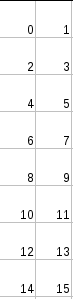
\includegraphics{minpillar}
    
    \subsubsection{SOL files}
    SOL files have not been fully figured out, however they are used becuase we can get some useful information out of them.
    Each byte in the SOL file is a bit field correcponding to an entry in the MIN file. Currently the only known value is the least signifigant bit, which indicates if a block is "passable" by the player and npcs (ie ground is passable, a wall isn't). A 0 in this position indicates that the block is passable, a 1 that it is not.

\newpage

\bibliographystyle{plain}
\bibliography{references}



\end{document}
